\section{Quadratic Splines}

A \textit{quadratic spline} is a set of piecewise quadratic functions which intersect all points in a dataset. There are three conditions that mathematically govern these functions. The first condition is that the functions must be \textit{continuous}. The second condition is that the functions must be \textit{smooth}, meaning that the derivatives are continous.

\begin{center}
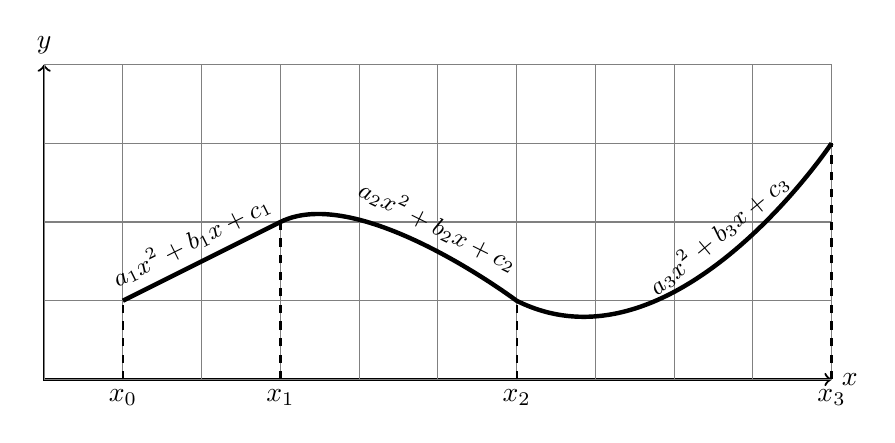
\begin{tikzpicture}
% Draw axes
\draw [<->,thick]
        (0,4) node (yaxis) [above] {$y$} |-
        (10,0) node (xaxis) [right] {$x$};
        
% Draw grid
\draw[gray, step=1cm] (0,0) grid (10,4);

% Draw path through points
        \draw [ultra thick]
        (1,1) -- 
        node[midway,above,sloped]
        {\small $a_1x^2+b_1x+c_1$}
        (3,2) .. controls (4,2.5) and (6,1) ..
        node[midway,above,sloped]
        {\small $a_2x^2+b_2x+c_2$}
        (6,1) .. controls (8,0) and (10,3) ..
        node[above,sloped]
        {\small $a_3x^2+b_3x+c_3$}
        (10,3);


% write x_0, x_1...
\draw[thick,dashed]
        (1,0) 
        node[below]{$x_0$} -- 
        (1,1);
\draw[thick,dashed]
        (3,0) 
        node[below]{$x_1$} -- 
        (3,2);
\draw[thick,dashed]
        (6,0) 
        node[below]{$x_2$} -- 
        (6,1);
\draw[thick,dashed]
        (10,0)
        node[below]{$x_3$} -- 
        (10,3);

% Draw points
\poi{1}{1}
\poi{3}{2}
\poi{6}{1}
\poi{10}{3}

\end{tikzpicture}
\end{center}

\subsection{Continuous Functions}
The spline equations should be continuous and go through all the points in the dataset. This means that the 

\begin{align}
f(x)
=
\begin{cases}
a_1x^2 + b_1x + c_1 & x_0 < x < x_1\\
a_2x^2 + b_2x + c_2 & x_1 < x < x_2\\
a_3x^2 + b_3x + c_3 & x_2 < x < x_3\\
\end{cases}
\end{align}

\subsection{Smooth Functions}


\begin{pseudocode}
\item Define dataset or take dataset as input if programmed as a stand alone function
\item Initialize $\vec{A}$ as a matrix of zeros (3n,3n)
\item Loop through number of points and use continuous function information

\begin{enumerate}
\item Set values for first equation
\end{enumerate}

\item Loop through number of points and use continuous derivatives information
\begin{enumerate}
\item Use interior points
\end{enumerate}

\end{pseudocode}